%!TeX root = thesis-main.tex
\chapter{Reinforcement Learning}\label{chap:marl}\mtcaddchapter

\minitoc% Creating an actual minitoc
\newcommand{\RS}{\mathcal{S}}
\newcommand{\RA}{\mathcal{A}}
\newcommand{\RP}{\mathcal{P}}
\newcommand{\RR}{\mathcal{R}}
\newcommand{\RE}{\mathbb{E}}

The concept of intelligence is as complex as it is intriguing, 
 and it has been a subject of philosophical inquiry, 
 scientific exploration, and cultural curiosity for centuries. 
 Philosophers have debated on what constitutes intelligence, 
 linking it to \emph{reason}, \emph{wisdom}, and even \emph{morality}. 
%
Despite these varied interpretations, 
 defining intelligence remains a challenge, 
 even in the field of psychology. 
%
Several standardized tests and scales attempt to measure intelligence,
 like the one developed by Alan Turing~\cite{Turing1950-TURCMA}, 
 but none manage to capture the complete essence of what it means to be ``intelligent''. 
 Intelligence is often understood as the ability to \emph{learn}, \emph{reason}, and \emph{adapt}, among other cognitive abilities.

Among the myriad of perspectives on intelligence, 
 learning stands out as a \emph{fundamental} component. 
 From an evolutionary point of view, 
 the ability to learn is essential for survival. 
 An organism that can adapt to its environment and learn from experiences is likely to survive and reproduce. 
 In the human context, learning has been the cornerstone of development, 
 be it mastering a language, solving complex problems, or creating art.

This notion of learning is crucial in the realm of Artificial Intelligence (AI). 
%
 If intelligence involves learning, 
 then replicating intelligence \emph{artificially} would necessarily entail enabling machines to learn. 
 This hypothesis leads us to the exciting and rapidly evolving domain of \emph{machine learning}---
 a subset of AI that allows computers to learn from data, 
 rather than requiring them to be explicitly programmed for specific tasks.

Machine learning encompasses various approaches and techniques that aim to make machines learn. 
 Broadly, these approaches can be categorized into supervised, 
 unsupervised, semi-supervised, and reinforcement learning.
%
Particularly, the first three approaches are based on the idea of \emph{learning from data}, 
 where this data can be labelled or unlabelled:
\begin{itemize}
  \item \emph{supervised learning}: this is the most straightforward approach, where a model is trained on a labelled dataset. 
  The model makes predictions or decisions based on input data, 
  and it is corrected when its predictions are incorrect. 
  Typical examples include classification and regression problems;
  \item \emph{unsupervised learning}: unlike supervised learning, this approach does not involve labelled data. 
  The machine tries to learn the patterns and the structure from the data without any supervision (e.g., clustering algorithms);
  \item \emph{semi-supervised}: A middle-ground between supervised and unsupervised learning, this approach utilizes both labelled and unlabelled data for training. 
  The model learns to improve its predictions gradually.
\end{itemize}
Reinforcement learning sets itself apart from other methodologies 
 by operating without the need for labelled data or supervision and through a sequential interaction between an agent and an environment employing a \emph{trial-and-error} strategy. 
 Subsequent sections will delve into the nuances of this distinctive approach, 
 starting from single-agent settings and then moving to multi-agent and many-agent systems.
\section{Single-agent}\label{chap:rl:single}
\begin{figure}
  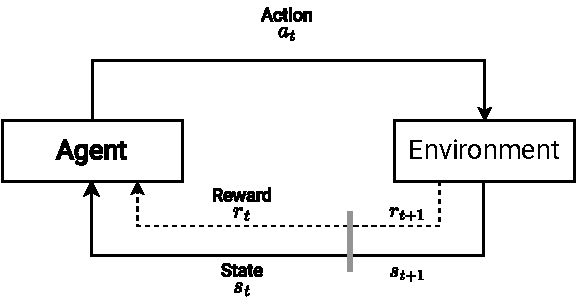
\includegraphics[width=\textwidth]{chapters/img/single-agent-rl.drawio.pdf}
  \caption{Overview of the \ac{rl} framework.}\label{fig:rl:overview}
\end{figure}
\Acl{rl}~\cite{sutton-book} serves as a universal framework 
 that has been inspired by the cognitive processes underlying human learning. 
 This paradigm has proven to be highly effective for addressing \emph{control problems}, 
 which are essentially tasks that require decision-making to achieve a particular outcome.
%
The core focus of \ac{rl} is on the \emph{sequential} interactions that occur between an \emph{agent} 
 and an \emph{environment} (summarized in \Cref{fig:rl:overview}). 
 Agents are defined as entities capable of performing \emph{actions}, 
 while the environment constitutes everything external to the agents 
 and beyond their immediate control.

During each discrete time step, denoted as $t$, 
 an agent observes the current state of the environment $s_t$ 
 (e.g., the robot position according to a GPS sensor). 
This state encapsulates the set of all observable information at that particular moment. 
The agent then proceeds to select an \emph{action} $a_t$ (e.g., the torque to be applied to engines) 
  in accordance with its \emph{policy} $\pi$. 
A policy serves as a probabilistic mapping that guides the agent in choosing actions 
 based on the current state. 
 Policies can be simple lookup tables or complex neural networks.
%
As a result of taking this action, 
 the environment transitions to a new state $s_{t+1}$ at the next time step $t+1$. 
 Simultaneously, the agent receives a \emph{reward} $r_{t+1}$, 
 which is a quantitative measure of the efficacy of the action taken, 
 given the state of the environment.

The overarching objective of \ac{rl} is to discover an \emph{optimal} policy, 
 denoted as $\pi^*$, that aims to maximize the long-term return, or cumulative reward, $G$. 
 This is generally achieved through a \emph{trial-and-error} learning process, 
 where agents continually adapt their policies based on the rewards received.

This framework has found extensive applications in a diverse array of domains. 
 For example, \ac{rl} has been used to create advanced algorithms for video games~\cite{DBLP:journals/spm/ArulkumaranDBB17}, 
 allowing for AI agents that can outperform human players. 
% 
In robotics~\cite{DBLP:journals/ijrr/KoberBP13}, 
 \ac{rl} algorithms are enabling machines to learn complex tasks autonomously, 
 from simple object manipulation to navigation in unstructured environments. 
 It is also making significant inroads in networking, 
 particularly in routing algorithms where dynamic decision-making is crucial~\cite{DBLP:journals/comsur/LuongHGNWLK19}.

\subsection{Markov Decision Process}
This general framework is supported by \ac{mdp}~\cite{howard1960dynamic}---
 a mathematical model that describes the environment evolution in sequential decision problems. 
%
A \ac{mdp} consists of a tuple $<\RS, \RA, \RP, \RR>$ in which:
\begin{itemize}
  \item $\RS$ denotes the set of states;
  \item $\RA$ is the set of actions;
  \item $\RP(s_{t + 1} | s_t, a_t)$ define the probability to reach some state $s_{t + 1}$ starting from $s_t$ and performing $a_t$ (i.e. transition probability function);
  \item $\RR(s_t, a_t, s_{t+1})$ devise a probabilistic reward function.
\end{itemize}
In \ac{mdp}, $\RP$ is \emph{memory-less}, 
 namely the next environment state depends only on the current state---
 that is the \emph{Markov property}.
%%
Another important concept in \ac{mdp} is the return 
 $G$ defined as the discounted sum of reward a possible future trajectory $\tau$ (i.e. a sequence of time steps):
%%
\begin{equation}
G_{t} = r_t + \gamma r_{t + 1} + \gamma^2 r_{t + 2} + \dots + \gamma^T r_{t + T} = \sum_{k = t}^T \gamma^{k-t} r_k
\end{equation}
%%
Where $0 \leq \gamma \leq 1$ is the \emph{discount factor}, 
 that is how much the future reward impacts the long-term return.
%%
Based on the value of $T$, 
 we can distinguish between \emph{episodic} and \emph{continuous} tasks.
 The foster ones are characterized by a finite number of time steps (e.g., a match of chess), 
 while the latter ones are infinite (e.g., a robot that should wander in an unknown environment).
%%
\subsubsection*{Reinforcement learning goal}
The \ac{rl} goal can be expressed as the maximization of the \emph{expected} 
 long-term return following a policy $\pi$:
%%
\begin{equation}
J = \mathbb{E_\pi}\Big[ G_t \Big] = \RE_\pi \Big[ \sum_{k = t}^T \gamma^{t-k} r_k \Big] 
\end{equation}
%%
Particularly, in \ac{RL} we want to find the optimal policy $\pi^*$ that maximizes $J$:
%%
\begin{equation}
\pi^* = \arg \max_{\pi} J
\end{equation}
The equation essentially captures the trade-off between immediate and future rewards. 
 The agent aims to select actions based on the policy \(\pi\) 
 that will maximize this expected long-term return. 
 The discount factor \(\gamma\) allows us to model the agent's consideration 
 for future rewards and is a hyperparameter that can be tuned based on the specific problem being solved.

\subsection{Find a policy given an MDP}
In the context of MDP, 
 evaluating policies is crucial for identifying the optimal one. 
 Consequently, two essential concepts are introduced: 
 the \emph{value function} and the \emph{Q-function}.
$V^\pi$ is the value function that evaluates how good (or bad) a \emph{state} 
 is according to the long-term return following the policy $\pi$ (\emph{expected value}).
% 
It is defined as:
%%
\begin{equation}
V(s)^\pi = \RE_\pi \Big[ G_t | s_t = s \Big]
\end{equation}
%%
$Q^\pi$ is the corresponding value function that evaluates \emph{state-action} pairs:
%%
\begin{equation}
Q(s, a)^\pi = \RE_\pi \Big[ G_t | s_t = s, a_t = a \Big]
\end{equation}
Policies could be defined through value functions. 
 In particular, a greedy policy based on $Q$ function is the one that always chooses 
 the action with the highest value in a certain state:
\begin{equation}
\pi(s) = \arg \max_{a}(Q(s, a))
\end{equation}
\subsubsection{Dynamic programming}
\begin{figure}
  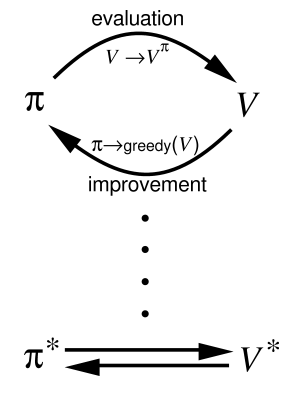
\includegraphics[width=0.3\textwidth]{chapters/img/generalized-policy-improvement.png}
  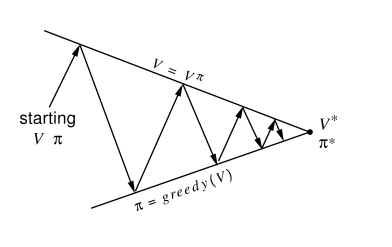
\includegraphics[width=0.65\textwidth]{chapters/img/value-iteration.png}
  \caption{General schema of policy iteration (left) and value iteration (right).}\label{fig:rl:dp}
\end{figure}
Dynamic programming is a family of algorithms that can be used to compute optimal policies 
 given a model of the environment as an \ac{mdp}.
%
In particular, the \emph{Bellman equation} is a fundamental concept in dynamic programming. 
 It is a recursive equation that decomposes the value function into two parts: 
 the immediate reward obtained from the current state and the discounted value of the future state. 
 The Bellman equation for the value function is defined as:
\begin{equation}
V(s) = \sum_{a \in \RA} \pi(a|s) \sum_{s' \in \RS} \RP(s'|s, a) \Big[ \RR(s, a, s') + \gamma V(s') \Big]
\end{equation}
%
Similarly, the Bellman equation for the $Q$ function is defined as:
\begin{equation}
Q(s, a) = \sum_{s' \in \RS} \RP(s'|s, a) \Big[ \RR(s, a, s') + \gamma \sum_{a' \in \RA} \pi(a'|s') Q(s', a') \Big]
\end{equation}
%
The Bellman equation is the basis for many algorithms that solve \ac{mdp},
two most notable are \emph{value iteration} and \emph{policy iteration} (\Cref{fig:rl:dp}).
\subsubsection{Value iteration}
Value iteration is an iterative algorithm used to compute the optimal value function \(V^*\) and,
 consequently, the optimal policy \(\pi^*\). 
 The algorithm is particularly useful when the state and action spaces are too large to solve directly through analytical methods. 
 It is based on the principle of optimality, which states that if an optimal policy \(\pi^*\) exists, then it must satisfy the Bellman optimality equation.

The algorithm starts by initializing \(V(s)\) 
 for all states \(s\) to some arbitrary values, often zeros. 
 It then iteratively updates the value of each state \(s\) 
 using the Bellman optimality equation until the value function converges to \(V^*\). 
 The convergence is usually checked by measuring the difference between successive value functions and comparing it against a small threshold \(\epsilon\):
\begin{equation}
V_{k+1}(s) = \max_{a \in \mathcal{A}} \sum_{s' \in \mathcal{S}} \RP(s'|s, a) \Big[ \RR(s, a, s') + \gamma V_k(s') \Big]
\end{equation}

The \(\max\) operation ensures that the value function is updated to reflect the best possible action at each state. 
 The term \(\gamma V_k(s')\) represents the discounted future rewards, 
 and \(R(s, a, s')\) is the immediate reward. 
 The transition probability \(P(s'|s, a)\) models the uncertainty in the environment.

After the value function has converged to \(V^*\), 
 the optimal policy \(\pi^*\) can be extracted. 
 The policy is determined by selecting the action that maximizes the expected return in each state, as given by:

\begin{equation}
\pi^*(s) = \arg \max_{a} \sum_{s' \in \mathcal{S}} P(s'|s, a) \Big[ R(s, a, s') + \gamma V^*(s') \Big]
\end{equation}
This policy is guaranteed to be optimal concerning the original MDP.

\subsubsection{Policy Iteration}
Policy iteration is another dynamic programming algorithm used for finding the optimal policy \(\pi^*\). 
 Unlike value iteration, policy iteration consists of two main steps: 
 \emph{policy evaluation} and \emph{policy improvement}, 
 which are repeated iteratively until the policy converges to \(\pi^*\):
\begin{itemize}
  \item policy evaluation: in this step, 
   the value function \(V^\pi\) for the current policy \(\pi\) is computed until it stabilizes. 
   The update rule is:
  \begin{equation}
  V_{k+1}(s) = \sum_{a \in \mathcal{A}} \pi(a|s) \sum_{s' \in \mathcal{S}} P(s'|s, a) \Big[ R(s, a, s') + \gamma V_k(s') \Big]
  \end{equation}
  \item policy improvement: after evaluating \(V^\pi\), 
  the policy is updated to be greedy with respect to \(V^\pi\):
  \begin{equation}
  \pi'(s) = \arg \max_{a} \sum_{s' \in \mathcal{S}} P(s'|s, a) \Big[ R(s, a, s') + \gamma V^\pi(s') \Big]
  \end{equation}
\end{itemize}
The algorithm then returns to the policy evaluation step, 
 using the new policy \(\pi'\), and continues until the policy no longer changes.

\subsection{Find a policy without an MDP}
While dynamic programming methods like value iteration and policy iteration offer powerful ways to find the optimal policy \(\pi^*\), 
 they come with a significant limitation: 
 the need for a complete model of the environment. 
 Specifically, these algorithms require knowledge of the transition probability function \(\RP\) and the reward function \(\RR\). 
%
In many real-world applications, 
 these functions are either unknown or too complex to model accurately. 
 This is where \emph{model-free} algorithms come into play.
 In the following sections, we will discuss two such algorithms' families: 
 Monte Carlo methods and Temporal Difference methods.
\subsubsection{Monte Carlo methods}
Monte Carlo methods offer a way to find an optimal policy \(\pi^*\) without requiring a model of the environment. 
 These methods rely on sampling sequences of states, actions, and rewards from actual or simulated interactions with the environment. 
 By averaging these samples, the agent can estimate the value functions \(V(s)\) and \(Q(s, a)\), which can then be used to improve the policy.

The core idea is to run multiple episodes, 
 from start to finish, and then update the value estimates based on the returns observed. 
 The value of a state \(s\) or a state-action pair \((s, a)\) is estimated as the average of the returns that have followed that state or state-action pair across multiple episodes.

\begin{equation}
V(s) = \frac{1}{N} \sum_{i=1}^{N} G_t^{(i)}
\end{equation}

\begin{equation}
Q(s, a) = \frac{1}{N} \sum_{i=1}^{N} G_t^{(i)}
\end{equation}

Where \(N\) is the number of times the state or state-action pair has been visited, 
 and \(G_t^{(i)}\) is the return following the \(i\)-th visit.

Once the value functions are estimated, 
 the policy can be improved by making it greedy concerning these estimated values. 
%
In this context, the \emph{exploration-exploitation} trade-off is crucial.
%
In fact, the agent should explore the environment to discover new states and actions that could lead to higher rewards,
  but it should also exploit the knowledge it has already acquired to maximize the expected return.
%
Monte Carlo methods are particularly useful when the state and action spaces are large, 
 making it impractical to enumerate all possible state-action pairs. 
 However, they do require the episodes to be finite and can be computationally expensive due to the need for multiple samples to obtain accurate estimates.

\paragraph*{The Exploration-Exploitation Dilemma in Reinforcement Learning}
The exploration-exploitation trade-off is a cornerstone challenge in reinforcement learning algorithms. 
 An agent must \emph{explore} its environment 
 to uncover new states and actions that may yield higher rewards. 
% 
Simultaneously, 
 it needs to \emph{exploit} its existing knowledge to maximize the expected return. 
 While this challenge pervades many learning algorithms, 
 it is especially prominent in model-free methods 
 where the agent learns a policy without having a predefined model of the environment.

Various strategies exist to navigate this dilemma. 
 One of the most prevalent is the \emph{$\epsilon$-greedy} policy. 
 In this approach, the agent selects a random action with probability \(\epsilon\) and 
 the action that is currently estimated to be the best with probability \(1 - \epsilon\). 
%
The \(\epsilon\) value is generally initialized to a small constant, such as 0.1 or 0.2, 
 to ensure a reasonable balance between exploration and exploitation. 
 Mathematically, the policy is defined as follows:
\begin{equation}
\pi(a|s) = \begin{cases}
\frac{\epsilon}{|\mathcal{A}|} + 1 - \epsilon & \text{if } a = \arg \max_{a \in \mathcal{A}} Q(s, a) \\
\frac{\epsilon}{|\mathcal{A}|} & \text{otherwise}
\end{cases}
\end{equation}

A useful refinement of the \(\epsilon\)-greedy strategy is to implement a \emph{decaying} \(\epsilon\), 
 which starts at a higher value and is reduced over time. 
 This adaptive approach allows the agent to initially focus on exploration to a greater extent, 
 then gradually shift toward exploiting its accumulated knowledge as its value function estimates stabilize.

\subsubsection{Temporal difference methods}
Temporal difference methods are a class of \emph{model-free} and \emph{value-based} algorithms 
 that allow the agent to learn optimal behaviour directly from its interactions with the environment, without requiring a model. 
 TD methods combine ideas from both Monte Carlo methods and dynamic programming to provide a flexible and powerful approach to reinforcement learning.

One of the simplest TD methods is \emph{TD-Learning}~\cite{DBLP:journals/ml/Sutton88}, 
 which updates the value function \(V(s)\) based on the temporal difference error \(\delta\), 
 defined as \( \delta = R(s, a, s') + \gamma V(s') - V(s) \). 
 The value function is then updated using \( V(s) \leftarrow V(s) + \alpha \delta \), where \(\alpha\) is the learning rate.

Starting from this intuition two main approaches have been developed: 
 \emph{Q-learning}~\cite{DBLP:journals/ml/WatkinsD92} and \emph{SARSA}~\cite{sutton-book}. 

 \paragraph*{Q-Learning}
 Q-Learning is an off-policy TD algorithm that focuses on learning the action-value function \(Q(s, a)\). The update rule for Q-Learning is:
 \begin{equation}
 Q(s, a) \leftarrow Q(s, a) + \alpha \Big[ R(s, a, s') + \gamma \max_{a'} Q(s', a') - Q(s, a) \Big]
 \end{equation}
 The algorithm is termed ``off-policy'' because it learns the value of the optimal policy regardless of the policy being followed, 
  thanks to the \(\max_{a'}\) term in the update rule.
 
The Q-Learning algorithm is guaranteed to converge to the optimal action-value function \(Q^*(s, a)\) as long as all state-action pairs are visited infinitely often and the learning rate \(\alpha\) is sufficiently small.
% 
For the same reason of decay \(\epsilon\)-greedy policy,
  it is also common to use a decaying learning rate, 
  which starts at a higher value and is reduced over time.
The full algorithm can be found in \Cref{alg:q-learning}.
\begin{algorithm}
\DontPrintSemicolon
\caption{Q-Learning}\label{alg:q-learning}
Initialise: $Q(s, a) = 0$ for all $s \in S$, $a \in A$\;
\Repeat{for every episode}{
    \For{$t = 0, 1, 2, \dots$}{
        Observe current state $s^t$\;
        \eIf{With probability $\epsilon$}{
            Choose random action $a^t \in A$\;
        }{
            Choose action $a^t \in \arg\max_a Q(s^t, a)$\;
        }
        Apply action $a^t$, observe reward $r^t$ and next state $s^{t+1}$\;
        $Q(s^t, a^t) \leftarrow Q(s^t, a^t) + \alpha \left[ r^t + \gamma \max_a Q(s^{t+1}, a) - Q(s^t, a^t) \right]$\;
    }
}
\end{algorithm}

 \paragraph*{SARSA}
 SARSA (State-Action-Reward-State-Action) is an on-policy TD algorithm. 
  Unlike Q-Learning, SARSA takes into account the current policy \(\pi\) during the learning process. The update rule for SARSA is:
 \begin{equation}
 Q(s, a) \leftarrow Q(s, a) + \alpha \Big[ R(s, a, s') + \gamma Q(s', a') - Q(s, a) \Big]
 \end{equation}
 where \(a'\) is the action taken under the current policy \(\pi\).
 
 Both Q-Learning and SARSA have their advantages and disadvantages. 
  Q-Learning tends to find the optimal policy faster but may be more sensitive to noise. 
  SARSA, being an on-policy method, is more conservative and tends to find safer policies, 
  especially when the policy involves some level of risk or uncertainty.

\subsection{Policy Gradient Methods}

While temporal difference methods and Monte Carlo methods focus on learning value functions to derive optimal policies, 
 \emph{policy gradient} methods take a different approach. 
%
They aim to directly optimize the policy \(\pi\) itself, 
 rather than first estimating value functions. 
%
This is particularly useful in environments with high-dimensional action spaces, 
 or continuous action spaces, where value-based methods may struggle.
%
Moreover, in this way, it is possible to learn stochastic policies,
 which are often more robust and flexible than deterministic policies.

Policy gradient methods optimize the policy by ascending the gradient of the expected return concerning the policy parameters \(\theta\). 
Mathematically, this can be expressed as:
\begin{equation}
\theta \leftarrow \theta + \alpha \nabla_\theta J(\theta)
\end{equation}
where \(J(\theta)\) is the expected return when following policy \(\pi_\theta\), 
 and \(\alpha\) is the learning rate.

One of the foundational algorithms in this category is the REINFORCE algorithm~\cite{DBLP:conf/nips/SuttonMSM99}: 
 it is one of the earliest and most straightforward policy gradient methods. 
It estimates the gradient of the expected return by sampling trajectories from the current policy \(\pi_\theta\). 
After each episode, the algorithm adjusts the policy parameters \(\theta\) in the direction that increases the expected return.
%
The core equation for the REINFORCE algorithm is:
\begin{equation}
\nabla_\theta J(\theta) = \mathbb{E}_{\tau \sim \pi_\theta} \left[ \sum_{t=0}^{\infty} \nabla_\theta \log \pi_\theta(a_t | s_t) G_t \right]
\end{equation}

Here, \(\tau\) represents a trajectory sampled from the policy \(\pi_\theta\), 
 and \(G_t\) is the return from time \(t\). 
A trajectory, or episode, is defined as a sequence of states, actions, and rewards.
%
The term \(\nabla_\theta \log \pi_\theta(a_t | s_t)\) is the log-likelihood gradient, 
 and \(G_t\) serves as a sample estimate for how good the action \(a_t\) is in state \(s_t\).

The REINFORCE algorithm operates in an episodic setting, 
 meaning it waits until the end of each episode to update the policy. 
 This makes it well-suited for tasks where the episode termination is natural, 
 such as games or tasks with a fixed time horizon.
%
REINFORCE is particularly useful when the action space is high-dimensional or continuous, 
 where traditional value-based methods like Q-Learning may struggle.  
 However, one drawback of REINFORCE is that it can have high variance in its updates, 
 which can make the training process unstable. 
%
Various techniques, such as using a \emph{baseline} 
 or employing advanced variance reduction methods, have been developed to mitigate this issue.
 Particularly, the \emph{actor-critic} architecture is a popular approach that combines the advantages of both value-based and policy-based methods.
 In this paradigm, the policy is referred to as the \emph{actor}, while the value function is referred to as the \emph{critic}.
The actor is responsible for selecting actions, while the critic evaluates the actions taken by the actor.

One popular extension of REINFORCE is proximity policy optimization (PPO)~\cite{ppo}---the algorithm used for training the ChatGPT model. 
 PPO is a policy gradient method that aims to improve the stability of the training process. 
 It does so by limiting the size of the policy update at each iteration, 
 which prevents the policy from changing too much between updates. 
\subsection{Approximate Solutions}

While the fundamental algorithms discussed in previous sections provide a strong theoretical foundation for model-free RL, 
 they often fall short in real-world applications. 
 The primary challenges they face are:

\begin{itemize}
  \item \textbf{Curse of dimensionality}: The state and action spaces in practical problems can be so large that enumerating them becomes computationally infeasible.
  \item \textbf{Partial observability}: In many scenarios, the agent cannot fully observe the entire state of the environment, 
  making it difficult to make optimal decisions.
\end{itemize}
To illustrate the curse of dimensionality, 
 consider the seemingly simple game of Go. 
 The game's state space consists of \(2^{170}\) possible states, 
 a number so astronomical that it exceeds computational capabilities—especially when compared to the estimated \(10^{80}\) atoms in the observable universe.

Similarly, partial observability is a pervasive issue in real-world applications. 
 For example, a self-driving car perceives its environment through sensors, 
 offering only a limited, partial view of the world. 
 This restricted perspective can significantly impact the agent's ability to make optimal decisions.

Given these challenges, approximate solutions become not just desirable but often \emph{necessary}. 
 These solutions leverage function approximation techniques to estimate value functions or policies. 
 While they may sacrifice some theoretical convergence guarantees, 
 they offer a more practical approach to tackling complex, 
 high-dimensional, and partially observable problems commonly encountered in real-world applications.
%
In contemporary applications, neural networks have emerged as the go-to function approximators 
 due to their exceptional capability to approximate complex, 
 high-dimensional functions. 
%
Particularly, the combination of \emph{deep learning} and reinforcement learning has led to significant advancements in the field, 
 in the so-called area of \emph{deep reinforcement learning}.
 One of the first and most influential works in this area was the Deep Q-Learning (DQL) algorithm~\cite{DBLP:journals/corr/MnihKSGAWR13}, which will be discussed in the next section.
 \subsubsection{Deep Q-Learning}

 Deep Q-Learning represent a landmark innovation in the field of deep reinforcement learning, 
  effectively combining the strengths of Q-Learning with the function approximation capabilities of deep neural networks.
  DQL was initially designed to master a variety of Atari 2600 games and has since been adapted for various complex tasks.
 
 The core idea behind DQL is to use a neural network as a function approximation for the Q-function in Q-Learning. 
  The neural network, often referred to as the Q-network, 
  takes the environment state as input and outputs Q-values for each action.
%  
Mathematically, the Q-network aims to approximate the optimal Q-function \(Q^*(s, a)\) 
 as closely as possible.
\begin{equation}
Q(s, a; \theta) \approx Q^*(s, a)
\end{equation}
where \(\theta\) represents the parameters of the neural network.
%
However, directly applying neural networks to Q-Learning presents challenges, 
 primarily due to the correlation between consecutive experiences and the non-stationary nature of the data. 
 DQL addresses these issues through two key innovations:
\begin{itemize}
  \item \textbf{Experience replay}: DQL stores past experiences \((s, a, r, s')\) in a replay buffer and samples mini-batches randomly during training. 
  This decorrelates the data and leads to more stable training.
  \item \textbf{Target network}: DQN introduces a separate, 
  slowly updated target network to calculate the target Q-values, 
  reducing the overestimation bias and improving stability.
\end{itemize}
The Q-value update equation in DQL is:
\begin{equation}
Q(s, a; \theta) \leftarrow Q(s, a; \theta) + \alpha \Big[ r + \gamma \max_{a'} Q(s', a'; \theta^-) - Q(s, a; \theta) \Big]
\end{equation}
Where \(\theta^-\) are the parameters of the target network.
\subsection{Wrap up}
\begin{figure}
  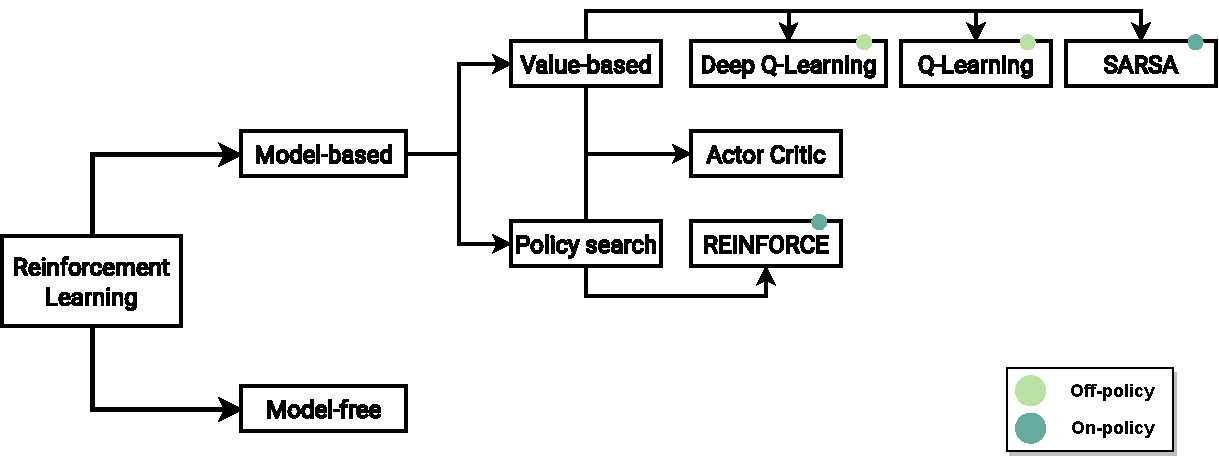
\includegraphics[width=\textwidth]{chapters/img/rl-overview.drawio.pdf}
  \caption{Overview of the \ac{rl} algorithms.}\label{fig:rl:overview}
\end{figure}
In conclusion, 
 this section has provided a comprehensive overview of RL, 
 beginning with the formulation of the problem and the underlying mathematical framework. 
 We also explored various analytical solutions and key algorithms associated with RL. 

Reinforcement learning algorithms can be categorized along multiple dimensions (summarized in \Cref{fig:rl:overview}). 
 One primary distinction is between \emph{model-free} and \emph{model-based} algorithms. 
 In the former, there is no need for a model of the environment, allowing the algorithm to learn directly through interaction. 
 In contrast, model-based algorithms require an MDP to compute the optimal policy.
%
Another important categorization is whether an algorithm is \emph{on-policy} or \emph{off-policy}. 
 On-policy algorithms optimize the same policy that is used for exploration, 
 whereas off-policy algorithms utilize two separate policies during the learning process, commonly referred to as the behaviour and target policies.
%
RL algorithms can be broadly divided based on what they aim to learn. 
 The primary categories here are value-based and policy gradient methods, 
 although hybrid approaches also exist that combine elements of both, like actor-critic.
%
Lastly, RL algorithms can be categorized based on whether they use a \emph{tabular} or \emph{approximate} approach. 
 Tabular methods store the value function in a table, 
 while approximate methods leverage function approximation techniques, 
 such as neural networks, to estimate the value function.

This overview serves as a basis for the multi-agent and many-agent RL algorithms,
 because most of the algorithms that we will discuss in the following sections are based on the concepts presented here.

\section{Multi-agent}
\begin{figure}
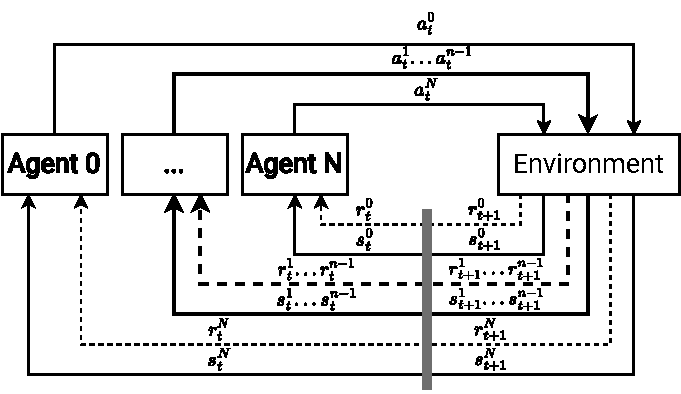
\includegraphics[width=\textwidth]{chapters/img/multi-agent-rl.drawio.pdf}
\caption{Overview of the \ac{marl} framework.}\label{fig:marl:overview}
\end{figure}
In the evolving landscape of \ac{rl}, 
 the concept of \acf{marl}~\cite{DBLP:conf/icml/Tan93,DBLP:journals/corr/abs-2108-02731,DBLP:journals/corr/abs-1908-03963} (\Cref{fig:marl:overview}) stands as a natural extension of the foundational \ac{rl} principles. 
 While traditional \ac{rl} generally focuses on the interactions between a single agent and an environment, 
 \ac{marl} broadens the scope to include multiple agents, 
 each with its own objectives, policies, and decision-making processes.

The basic setting in \ac{marl} comprises multiple agents interacting either \emph{cooperatively}, \emph{competitively}, or in a \emph{mixed} fashion within a shared environment---more details in the following sections. 
 Each agent $i$ observe its the environment state $s_{t}^{i}$, 
 select actions $a_{t}^{i}$ according to its policy $\pi^{i}$, 
 and receive rewards $r_{t+1}^{i}$.
 However, in \ac{marl}, 
 an agent's actions can directly or indirectly influence the states and rewards of other agents, 
 thereby increasing the complexity of the learning problem.
The key challenge in \ac{marl} 
 is to develop robust algorithms that enable agents to learn optimal policies in these complex, 
 often \emph{non-stationary}, environments. 
 Classic \ac{rl} algorithms often require modifications to accommodate the multi-agent setting. 
 For instance, the concept of a joint action space, a state space extended to multiple agents, 
 and a composite reward function are essential considerations.
\subsection{Stochastic games}
The formalization of MARL typically extends the standard Markov Decision Process (MDP) 
 framework to account for multiple agents. 
 One of the most straightforward extensions is the Markov Game, also called Stochastic games~\cite{neyman2003stochastic}. 
 In this formalization, 
each agent has its own state, action, and reward function, 
and the joint actions of all agents determine the transition dynamics and rewards: 
\begin{equation}
S = \langle \mathcal{N}, \mathcal{S}, \mathcal{A}_1, \ldots, \mathcal{A}_N, \mathcal{P}, \mathcal{R}_1, \ldots, \mathcal{R}_N \rangle
\end{equation}
Where:
\begin{itemize}
    \item $\mathcal{N}$ is the number of agents. 
    With $N=1$ we have a single-agent setting, while with $N >> 2$ we have a many-agent setting.
    \item $\mathcal{S}$ is the environment state space. The environment is then considered to be fully observable. 
    \item $\mathcal{A}_i$ is the action space of agent $i$. We denote the joint action space as $\mathbb{A} = \mathcal{A}_1 \times \ldots \times \mathcal{A}_N$.
    \item $\mathcal{P}: \mathcal{S} \times \mathbb{A} \rightarrow \Delta(\mathbb{S})$ is the joint transition probability function. 
    For each time step $t$, $\mathcal{P}$ is a function of the joint action $a_t \in \mathbb{A}$ and the current state $s_t \in \mathcal{S}$, 
    and returns the probability of transitioning to the next state $s_{t+1} \in \mathcal{S}$.
    \item $\mathcal{R}_i: \mathbb{S} \times \mathbb{A} \times \mathbb{S} \rightarrow \mathbb{R}: $ is the reward function for agent $i$. 
    The joint reward function is defined as $\mathbb{R} = \mathcal{R}_1 + \ldots + \mathcal{R}_N$.
\end{itemize}
The game can be described sequentially as follows:
\begin{enumerate}
    \item At each time step $t$, each agent $i$ observes the current state $s_t^i$.
    \item Each agent $i$ selects an action $a_t^i$ according to its policy $\pi^i$.
    \item The joint action $a_t = (a_t^1, \ldots, a_t^N)$ is executed, and the environment transitions to the next state $s_{t+1}$ according to the transition probability function $\mathcal{P}$.
    \item Each agent $i$ receives a reward $r_{t+1}^i$ according to the reward function $\mathcal{R}_i$.
\end{enumerate}
It is important to note that in these games, 
 actions from all agents are executed simultaneously, 
 and each agent's reward is a function of the joint action taken by all agents. 
%
In many real-world scenarios, assuming the availability of a global system state is impractical. 
 As such, an often-employed extension to the traditional Stochastic Game model is the \emph{Partially Observable Stochastic Game} (POSG)~\cite{li2022zero}. 
 This extension can be formally represented as follows:
\begin{equation}
\text{POSG} = \langle \mathcal{N}, \mathcal{S}, \mathcal{A}_1, \ldots, \mathcal{A}_N, \mathcal{P}, \mathcal{R}_1, \ldots, \mathcal{R}_N, \mathcal{O}_1, \ldots, \mathcal{O}_N, \mathcal{O} \rangle
\end{equation}
Here, 
 the primary divergence from the conventional Stochastic Game 
 is the introduction of observation functions \(\mathcal{O}_i: \mathcal{S} \rightarrow \mathcal{O}_i\), 
 which maps the environment state to the observation space of agent \(i\). 
 Consequently, the agents' policies are now parameterized by their respective observation spaces \(\mathcal{O}_i\) rather than the global state space \(\mathcal{S}\). 
 This alteration significantly influences both the algorithmic approaches and the complexities involved in solving POSGs.
\subsection{Taxonomies}
\begin{figure}
  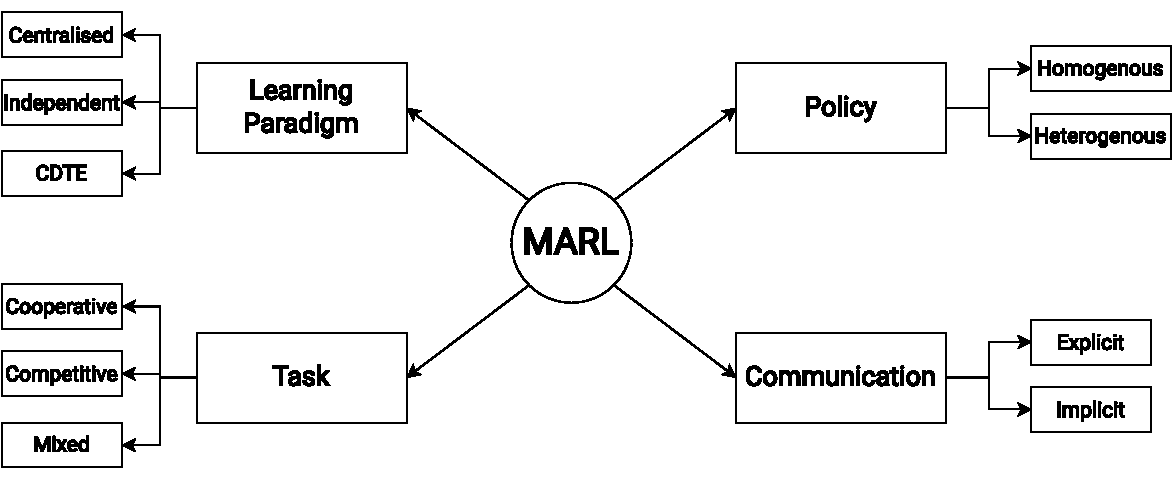
\includegraphics[width=\textwidth]{chapters/img/marl-taxonomy.drawio.pdf}
  \caption{Overview of the \ac{marl} taxonomies.}\label{fig:marl:taxonomy}
\end{figure}
In single-agent settings, the focus of learning configurations is primarily on \emph{algorithmic} aspects, 
 such as whether an approach is value-based or relies on policy search, 
 or whether it operates on-policy or off-policy. 
%
However, the landscape becomes more complex when multiple agents are involved. 
In such multi-agent settings, 
 several dimensions must be considered to appropriately classify algorithms and approaches. 
Various surveys~\cite{DBLP:journals/corr/abs-2108-02731,DBLP:journals/corr/abs-1908-03963} have attempted to categorize the diverse classes of algorithms specifically designed for multi-agent scenarios. 
Each of these surveys emphasizes a unique characteristic or aspect of the problem under consideration. 
%
This section endeavours to outline various dimensions along which multi-agent algorithms can be categorized (\Cref{fig:marl:taxonomy}). 
 The objective is to provide a framework for situating the algorithms that will be discussed in subsequent sections, 
 particularly those that pertain to the \emph{many-agent} perspective.
Note that the following taxonomies are not mutually exclusive, 
 and many algorithms can be classified along multiple dimensions.
\subsubsection{Learning Paradigms}
\begin{figure}
  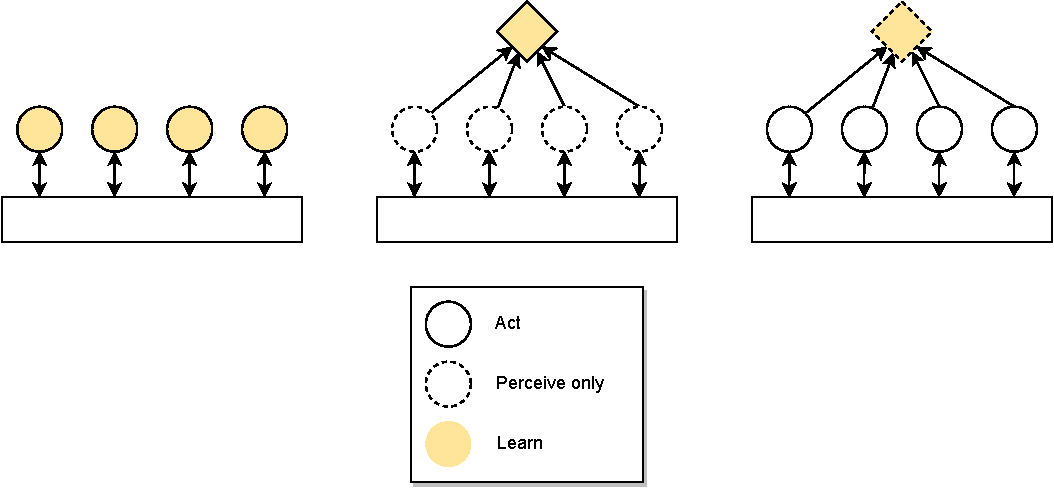
\includegraphics[width=\textwidth]{chapters/img/marl-policy-kind.drawio.pdf}
  \caption{Overview of the \ac{marl} learning paradigms.}\label{fig:marl:policy-kind}
\end{figure}
\sloppy
One possible categorization of multi-agent algorithms is based on the learning paradigm (summarized in \Cref{fig:marl:policy-kind}). 
 In this context, the learning paradigm refers to how agents learn their policies. 
The field of multi-agent learning has historically been dominated by two primary approaches: 
 \emph{independent learning} and \emph{centralized learning}. 
 In independent learning, 
 each agent learns its own policy concurrently and independently of the other agents in the environment~\cite{tan1993multi}. 
 In contrast, centralized learning involves a single learning entity that constructs a joint policy to control all agents.
 
Independent learning excels in scalability but often results in unstable learning dynamics due to the non-stationarity of the environment. 
This non-stationarity stems from the concurrent learning of multiple agents, 
 making it challenging to learn effective policies. 
%
On the other hand, centralized learning benefits from environmental stability owing to the global view it maintains. 
 However, it suffers from scalability issues due to the exponential growth of the state and action spaces as the number of agents increases.
%
To illustrate, consider a system comprising \( N \) agents, 
 each capable of taking \( M \) actions. 
 In a centralized framework, the number of possible joint actions would be \( M^N \). 
 For instance, with \( N=100 \) and \( M=2 \), the number of joint actions would be an astronomical \( 2^{100} \).

Recognizing the limitations of both independent and centralized learning paradigms, 
 recent research has proposed a compromise: 
 Centralized Training with Decentralized Execution (CTDE)~\cite{DBLP:conf/nips/LoweWTHAM17}. 
 In this approach, agents are trained using a \emph{global} view of the environment to learn a distributed policy. 
 Indeed, during execution, each agent relies solely on its \emph{local} observations to select actions. 
 This hybrid method is particularly advantageous in partially observable environments: 
 agents can learn a policy influenced by global states during the training phase while requiring only local observations for decision-making during execution.

\subsubsection{Task type}
Aside how the agent learns, 
 another important distinction involves \emph{what} the agent should learn.
%
The task type can be \emph{cooperative}, \emph{competitive}, or \emph{mixed}.
\paragraph*{Cooperative}
In cooperative tasks, 
 agents are geared towards a common objective, 
 aiming to maximize a shared reward. 
 Formally, this is represented as a unified reward function for all agents, given by:
\begin{equation}
\mathcal{R}_0 = \mathcal{R}_1 = \ldots = \mathcal{R}_N = \mathcal{R}
\end{equation}
Here, the objectives of all agents are perfectly aligned, 
 necessitating coordination and collaboration among them to achieve the shared goal. 
 Such cooperative scenarios are often encountered in the domain of \ac{cpsw}, 
 where inter-agent coordination is crucial for realizing collective outcomes effectively and efficiently.
\paragraph*{Competitive}
In competitive tasks, agents operate under divergent objectives, 
 and the reward function is usually tailored to each agent's performance. 
This can be formally expressed in two-player games as:
\begin{equation}
\mathcal{R}_0 = -\mathcal{R}_1
\end{equation}
In this framework, the agents have conflicting goals, 
 creating a competitive landscape where each agent aims to maximize its reward. 
\paragraph*{Mixed}
In mixed tasks, agents operate under both cooperative and competitive dynamics. 
 This is often encountered in real-world scenarios, 
 where agents may have both shared and divergent objectives. 
This is the most general setting, and it is often the most challenging to solve.
\subsubsection{Policy type}
Another crucial aspect to explore is the nature of the policy that an agent ought to learn. 
Although numerous classifications of policies exist
 ---ranging from deterministic to stochastic, centralized to decentralized, and joint to individual---
 this thesis places special focus on distinguishing between \emph{homogeneous} and \emph{heterogeneous} policy family.

\paragraph*{Homogeneous Policies}
In the context of homogeneous policies, 
 all agents \emph{share} a common policy. 
 The learning process aims to identify a \emph{single}, \emph{unified} policy applicable to all agents. 
 This is particularly prevalent in cooperative tasks where agents must collaborate to achieve a collective objective. 
 Utilizing a single policy across all agents often simplifies the learning process and enhances coordination among the agents.
 Moreover, is particularly suitable for scenarios where agents are \emph{interchangeable} and \emph{indistinguishable}, 
 making it possible to use the same policy in different agent populations.
\paragraph*{Heterogeneous Policies}
Conversely, in the realm of heterogeneous policies, 
 each agent possesses its distinct policy. 
 The learning algorithm is tasked with discovering a unique policy tailored to each agent. 
 This approach, even if it can be also used in the context of cooperative tasks, 
 is especially useful in competitive environments, 
 where agents have disparate objectives and strive to optimize their rewards. 
 Employing unique policies for each agent allows for the development of diverse strategies and behaviours, 
 accommodating the complex dynamics of competitive settings.
\subsubsection{Communication}
Another important dimension to consider is whether agents are allowed to communicate with each other. 
 In many real-world scenarios, agents are capable of exchanging information with other agents in the environment. 
 This communication can be \emph{explicit}, 
 such as through the exchange of messages, or \emph{implicit}, 
 such as through the observation of other agents' actions. 

In contrast, in other scenarios, agents are not allowed to communicate with each other. 
 This is often the case in competitive settings, 
 where agents are not permitted to share information. 
 This restriction is often imposed to increase the complexity of the problem and to encourage the development of more sophisticated strategies.

\subsection{Solutions for MARL}
Addressing the intricacies and challenges inherent in \ac{marl} requires the design and implementation of sophisticated algorithms 
 and frameworks capable of navigating a complex landscape shaped by multi-agent interactions, 
 a diverse range of tasks, and varied learning paradigms. 
%
Over the years, a plethora of methodologies have emerged to confront these obstacles. 
 Specifically, this thesis provides a comprehensive overview of approaches rooted in the \ac{rl} domain.

A significant body of literature instead focuses on game-theoretical perspectives, 
 which predominantly address scenarios involving a limited number of agents engaged in competitive tasks. 
 Such approaches often incorporate concepts of \emph{equilibrium} and \emph{convergence} towards stable policies, 
 typically framed within the context of Nash equilibrium.
%
However, in practice, the pursuit of equilibrium often fails to yield satisfactory results, 
 as it does not necessarily lead to agents learning optimal policies. 
 Consequently, a substantial portion of the literature eschews equilibrium-centric views, 
 opting instead to develop algorithms aimed at effective policy learning, 
 even in the absence of formal proofs guaranteeing convergence to an equilibrium.

 \subsubsection{Tabular Methods}
The first era of \ac{MARL} 
 algorithms primarily relied on tabular methods, 
 based on variation of Q-Learning and SARSA. 
These methods are essentially extensions of single-agent tabular algorithms adapted for a multi-agent setting. 
In this section, we will briefly discuss some of the most popular tabular algorithms, 
 laying the groundwork for the discussion of more advanced approaches in subsequent sections.

 \paragraph*{Distributed Q-Learning} is a straightforward extension of the traditional Q-Learning algorithm designed for multi-agent systems. 
In this approach, 
 each agent maintains its own Q-table and updates it based on its local observations and rewards.
 while this method allows for decentralized learning, 
it often struggles with issues related to \emph{coordination} and \emph{convergence} to global optima. The algorithm is particularly useful in scenarios where communication between agents is limited or not possible.
However, it may not always guarantee convergence to the optimal joint policy, 
especially in complex environments where coordination between agents is crucial.
 
 \paragraph*{Hysteretic Q-Learning~\cite{hysteretic-q}} is a more recent addition to the family of tabular MARL algorithms. 
  It addresses some limitations of Distributed Q-Learning, 
  particularly in the context of cooperative multi-agent systems. 
  In Hysteretic Q-Learning, each agent employs \emph{two} learning rates for updating its Q-values, 
  depending on whether the received reward is better or worse than expected. 
  Formally, the update rule is:
  \begin{align*}
    \delta & \leftarrow r - Q_i(a_i) \\
    Q_i(a_i) & \leftarrow 
    \begin{cases} 
    Q_i(a_i) + \alpha \delta & \text{if } \delta \geq 0 \\
    Q_i(a_i) + \beta \delta & \text{else}
    \end{cases}
  \end{align*}
  This dual learning rate mechanism allows for more flexible and efficient coordination among agents. 
  Experimental results have shown that Hysteretic Q-Learning not only converges faster but also achieves comparable performance to centralized methods with significantly less computational overhead.

 \paragraph*{QD-Learning~\cite{qdlearning}}
 is a distributed version of the traditional Q-Learning algorithm tailored for multi-agent systems. 
%
Unlike centralized approaches, 
 QD-Learning allows agents to engage in the learning process autonomously through \emph{local} communication and computation.
% 
Each agent maintains a sequence of Q-matrices, 
  and the Q-values for each state-action pair evolve in a collaborative distributed manner. 
%
Specifically, the Q-values are updated according to a formula that incorporates both local one-stage costs 
  and information from neighbouring agents.

The primary objective of QD-Learning is to minimize a network-averaged infinite horizon discounted cost. 
%
The algorithm achieves this by ensuring 
 that each agent learns the value function based on locally 
 accessible stochastic processes and one-stage cost processes. 
%
The agents collaborate using local processing and mutual information exchange, 
 aiming to reach a consensus on the desired value function and the corresponding optimal control strategy.
%
In terms of performance, 
 QD-Learning has been shown to achieve optimal learning performance asymptotically, 
 under minimal connectivity assumptions on the underlying communication graph. 
%
It has also been found to have a negligible asymptotic
 convergence rate loss compared to centralized Q-Learning
 making it a robust choice for distributed multi-agent systems.
The update rule for QD-Learning is:
 \begin{align*}
  Q^n_{i,u}(t+1) &= Q^n_{i,u}(t) - \beta_{i,u}(t) \sum_{l \in \Omega_n(t)} (Q^n_{i,u}(t) - Q^n_{l,u}(t)) \\
  &\quad + \alpha_{i,u}(t) \left( c_n(x_t, u_t) + \gamma \min_{v \in U} Q^n_{x_{t+1},v}(t) - Q^n_{i,u}(t) \right)
  \end{align*}
 
 where \(\beta_{i,u}(t)\) and \(\alpha_{i,u}(t)\) are weight sequences adapted to the filtration \(\mathcal{F}_{n}(t)\), and \(c_{n}(x_{t}, u_{t})\) is the local one-stage cost.

\subsubsection{Approximate methods}
The tabular methods discussed in the previous section are often impractical in real-world scenarios, 
 as they require the storage of a Q-table for each agent. 
 This can be computationally infeasible, 
 especially in complex environments with large state and action spaces.
%
To address this issue, 
 a variety of approximate methods have been developed, 
 leveraging function approximation techniques to estimate the Q-values or policies.
%
The following are the most popular approximate methods for MARL, a complete overview however is out of the scope of this thesis and can be found in~\cite{DBLP:journals/corr/abs-1908-03963}. 
\paragraph*{Counterfactual Multi-Agent (COMA)~\cite{DBLP:journals/corr/FoersterFANW17}}
 is an actor-critic method specifically designed for cooperative multi-agent systems.
 Unlike traditional methods that rely on decentralized policies,
 COMA employs a centralized critic during the learning phase to estimate the Q-function. 
 This centralized critic takes into account the global state or the joint action-observation histories, 
 making it more effective in complex environments.

One of the key innovations in COMA is the introduction of a counterfactual baseline to address the challenge of multi-agent credit assignment. 
 In cooperative settings where joint actions produce global rewards, 
 it becomes difficult for individual agents to understand their contribution to the team's success. 
 The counterfactual baseline marginalizes a single agent's action while keeping the other agents' actions fixed, 
 thereby providing a more accurate estimate of each agent's contribution.
Another advantage of COMA is its computational efficiency.
 It employs a critic that allows the counterfactual baseline to be computed in a single forward pass, 
 thereby reducing the computational burden.

COMA has been evaluated in complex scenarios like StarCraft unit micromanagement and has shown significant improvements over other multi-agent actor-critic methods. 
 It is particularly useful in environments with high stochasticity, 
 large state-action spaces, and delayed rewards.

\paragraph*{Multi-Agent Proximal Policy Optimization (MAPPO)~\cite{mappo}}
 is an extension of the widely-used Proximal Policy Optimization (PPO) algorithm, 
 adapted for cooperative multi-agent systems. 
 Unlike traditional methods that often rely on off-policy learning algorithms, 
 MAPPO is an on-policy method that has shown to be surprisingly effective in multi-agent settings.

MAPPO employs a centralized value function during the training phase to estimate the Q-values.
%
 This centralized critic can take into account global state information, 
 allowing MAPPO to follow a CTDE structure. 
%
 This is particularly useful in complex environments where the state and action spaces are large, 
 as it allows for more effective policy updates.

One of the standout features of MAPPO is its \emph{sample efficiency},
 that means the ability to learn from a few samples. 
 Despite being an on-policy method, 
 MAPPO is competitive or 
 even superior to off-policy methods in terms of both final returns and sample efficiency. 
%
MAPPO also benefits from the robustness and stability of the underlying PPO algorithm. 
 It requires minimal hyperparameter tuning and does not necessitate any domain-specific algorithmic modifications or architectures to achieve strong performance. 
 This makes it a versatile and practical choice for a wide range of multi-agent environments.
\paragraph*{QMIX~\cite{QMIX}}
 is a value-based method designed to address the challenges in multi-agent reinforcement learning (MARL). 

It is based on the idea of \emph{factorisation}, 
 which involves decomposing the joint action-value function into a set of individual value functions. 
 This factorisation allows for the extraction of decentralized policies that are consistent with the centralized training.

The architecture of QMIX consists of individual agent networks and a mixing network. 
 Each agent network estimates an individual value function \( Q_a \), while the mixing network combines these into a joint action-value function \( Q_{\text{tot}} \). 
 A key feature of QMIX is the \emph{monotonicity} constraint, 
 which ensures that the joint action-value function is monotonic in the individual agent value functions. 
 This allows for the extraction of decentralized policies that are consistent with the centralized training.
%
QMIX is particularly effective in environments 
 where the joint action spaces grow exponentially with the number of agents. 
 It employs a mixing network with positive weights to enforce the monotonicity constraint, 
 thereby ensuring that decentralized policies can be easily extracted. 
 This makes QMIX computationally efficient and scalable, as it avoids the need for storing a Q-table for each agent.

\subsection{Wrap up}
In this section, we have provided an overview of \ac{marl} functional for this thesis perspective,
 beginning with the formulation of the problem and the underlying mathematical framework. 
 We also explored various analytical solutions and key algorithms associated with \ac{marl}.
In the following, we will discuss the \emph{many-agent} perspective, 
understanding the challenges and the solutions proposed in the literature.

\section{Many-agent}
\ac{cpsw} are characterized by a very large number of agents, 
 with a population that can potentially range from hundreds to millions of agents.
%
In such scenarios, 
 the traditional \ac{marl} framework is no longer applicable, 
 as the number of agents makes it computationally infeasible to learn a joint policy.
%
A novel approach is required to address the challenges of many-agent systems, 
 which is the focus of this section--in the so-called area of \ac{MAARL}~\cite{yang2021many}.
%
When we discuss many-agent systems, 
 we refer to a large number of agents ($N \gg 2$) 
 that are \emph{interchangeable} and \emph{indistinguishable}.
%
In \ac{cpsw} perspective, 
 it is still applicable because we consider the agent to be behavioural homogeneous, 
 even if they are not identical.

After this brief introduction, 
 we will discuss the peculiarities of many-agent systems,
 starting from the formalization of the problem,
  and then we will discuss practical solutions in this context.
\subsection{Formalization}
Standard stochastic games do not capture the essence of many-agent systems, 
 as they do not consider the homogeneous nature of the agents, and the large number of agents.
Therefore, in the context of swarm robotics, 
 a novel framework called \emph{SwarMDP}~\cite{vsovsic2016inverse} has been proposed.
 This is focused on the idea of having a \emph{swarming agent} that rules the entire population of agents.
 In the following, we will discuss the formalization of this framework.
Moreover, this model can be also applied in the system dynamics of aggregate computing discussed in \Cref{ssec:background:sysmodel}.
\subsubsection{SwarMDP}
A SwarMDP is characterized by a \emph{swarming agent} ($\mathbb{A}$) and the dynamics of the environment ($\mathbb{E}$).
Specifically, $\mathbb{A}$ is a tuple ($\mathcal{S}, \mathcal{O}, \mathcal{A}, \mathcal{R}, \pi$) where:
\begin{itemize}
  \item $\mathcal{S, O, A}$ are the set of local states, observations (or features), and actions, respectively;
  \item $\mathcal{R}: \mathcal{S} \rightarrow \mathbb{R}$ is the reward function, which is influenced by the environment;
  \item $\pi: \mathcal{O} \rightarrow \mathcal{A}$ is the policy function, which maps the observations to the actions: it could be deterministic or stochastic.
\end{itemize}
Starting from this definition, the environment $\mathbb{E}$ is defined as a tuple ($\mathcal{P}, \mathbb{A}, \mathcal{T}, \xi$), where:
\begin{itemize}
  \item $\mathcal{P}$ is the total number of agents in the systems (the agent population), which is assumed to be fixed;
  \item $\mathbb{A}$ is the defined agent prototype that rules each agent $v \in P$;
  \item $\mathcal{T}: \mathcal{S}^P \times \mathcal{A}^P \times \mathcal{S}^P \rightarrow \mathbb{R}$ is the transition  global function, which is influenced by the actions of the agents and returns a collective reward -- this is typically not known by the swarming agents;
  \item $\xi: \mathcal{S^P} \rightarrow \mathcal{O^P}$ is the global observation model of the systems.
\end{itemize}

\subsection{Solutions for \ac{MAARL}}
In a \ac{MAARL} scenario, 
 the concept of \emph{homogeneity} is leveraged to design algorithms that scale effectively with the number of agents. 
 Rather than developing $N$ distinct policies for $N$ agents, 
 the objective is to formulate a \emph{single} policy applicable to all agents.
%
The learning paradigm typically employed in this context is CDTE, for the following reasons:
\begin{itemize}
\item fully decentralized learning is impractical due to the high level of non-stationarity 
 that arises from concurrent learning.
\item An agent's view of the system is so limited that locally 
 collected experiences are insufficient for capturing the full range of possible local behaviour.
\end{itemize}
While several CDTE algorithms, such as MAPPO and QMIX, aim to find $N$ policies, 
 various practical adjustment can be employed to adapt them for multi-agent settings. 

Subsequently, we will discuss the most popular of these techniques, as well as algorithms specifically designed for many-agent systems.
\subsubsection*{Parameter sharing}
Parameter sharing~\cite{albrecht2023multi} is a pivotal technique in \ac{MAARL}, 
 due to the strongly homogeneous agent assumptions. 
% 
The essence of this approach lies in the utilization of a unified set of parameter values, 
 denoted as \( \theta_{\text{shared}} \) for the policy network or \( \phi_{\text{shared}} \) 
 for the value network, across all agents.
 This can be extended also to the case of standard \ac{rl} algorithms, 
 where the parameter sharing is applied to the Q-table. 
This unified parameter set serves as the backbone for both the policy and value functions of each agent.
This learning approach is effective in many-agent systems, and it has several advantages:
\begin{itemize}
  \item \textbf{Sample efficiency}: 
  one of the most compelling advantages is the improvement in sample efficiency. 
  By learning a single set of parameters, 
  the algorithm can generalize across agents, 
  thereby utilizing a more diverse and larger set of trajectories for training.
  \item \textbf{Computational efficiency}: 
  parameter sharing keeps the computational load manageable by maintaining a constant number of parameters, 
  irrespective of the number of agents. 
  This is in stark contrast to a non-shared approach, 
  where the number of parameters would increase linearly with the number of agents.
\end{itemize}
This, however, comes at the cost of policy space limitation: employing parameter sharing inherently constrains the policy space to identical policies for each agent, 
 reducing the complexity of the overall joint policy.
 Said that, in \ac{cpsw} this is quite reasonable,
 because complexity comes from the interaction of simple agents,
  rather than from complex agents.
 
Mathematically it involves constraining the policy parameters \( \theta \) and/or value function parameters \( \phi \) across agents as follows:
\[
\theta_{\text{shared}} \equiv \theta_1 \equiv \theta_2 \equiv \ldots \equiv \theta_N
\]
\[
\phi_{\text{shared}} \equiv \phi_1 \equiv \phi_2 \equiv \ldots \equiv \phi_N
\]
where \( N \) is the number of agents.

\subsubsection*{Experience Sharing}
Experience sharing serves as another cornerstone in \ac{MAARL}~\cite{albrecht2023multi}.
 Unlike parameter sharing, which centralizes the neural network parameters across agents, 
 experience sharing focuses on the distribution of experiences or trajectories among agents.
By pooling experiences from multiple agents into a shared replay buffer, 
 each agent has the opportunity to learn from a much richer set of experiences than it could generate on its own. 
 This not only speeds up the learning process but also ensures a more uniform learning progression across agents, which is particularly useful for tasks that require coordinated multi-agent actions.

However, experience sharing comes with its own set of challenges. 
 For instance, the approach can be computationally intensive as it increases the size of the batch used for training. Additionally, unlike parameter sharing, 
 experience sharing allows for the possibility of agents learning diverse policies. 
 However, these approaches can be combined to leverage the benefits of both techniques.

In terms of mechanics, 
 experience sharing typically involves storing each agent's experiences, 
 usually denoted as \( (s, a, r, s') \), in a shared replay buffer. 
 During the learning phase, agents sample from this shared buffer to update their individual policies and value functions. 

\subsubsection*{Many-agent Q-Learning}
Many-agent Q-Learning extends the classic Q-Learning algorithm to a multi-agent setting by incorporating the concepts of experience sharing and parameter sharing. 
 In this approach, each agent maintains a global Q-table but can learn from a shared experience replay buffer. 
 This shared buffer contains the state-action-reward-next state tuples \( (s, a, r, s') \) from all agents, 
 thereby enriching the learning process for each individual agent.
 
The algorithm operates similarly to traditional Q-Learning, 
 with the primary difference being the source of experiences used for updates. 
 During each learning iteration, agents sample experiences from the shared replay buffer to update the global Q-values. 
 The Q-value update equation remains the same as in single-agent Q-Learning, 
 but the experiences used for the updates are drawn from the collective experiences of all agents.
 
By leveraging shared experiences, 
 this approach aims to achieve faster convergence and more robust policies. 
 Agents benefit from the diverse set of experiences, which can be particularly useful in complex or stochastic environments where individual experiences may not provide sufficient coverage of the state-action space.
  
This method is especially useful in scenarios where agents are working towards a common goal but partial observability of the environment. 
 By sharing experiences, 
 they can collectively learn a more comprehensive and effective strategy to achieve their objective.
%
This can be also extended to deep-q learning approaches, 
 where the Q-table is replaced by a neural network.
%
\begin{algorithm}
\caption{Many-agent Q-Learning}
\label{alg:maql}
\DontPrintSemicolon
\KwData{Initialize a global value function with random Q}
\KwData{Initialize a single replay $D_{\text{shared}}$ buffer for all agents}
\KwData{Collect environment observations $o^0_1, \dots, o^0_n$}
\For{time step $t = 0, \dots, d$}{
    \For{agent $i = 1, \dots, n$}{
        \eIf{with probability $\varepsilon$}{
            choose random action $a_i$\;
        }{
            choose $a_i = \max_{a} Q(h_t, a_i)$\;
        }
        Execute actions and collect observations $o^{t+1}_i$ and rewards $r_i$\;
        Store all transitions in replay buffer $D_{\text{shared}}$\;
    }
    \For{agent $i = 1, \dots, n$}{
        Sample random mini-batch of transitions from replay buffer $D_{\text{shared}}$\;
        Update Q by the Bellman equation
    }
}
\end{algorithm}
The algorithm is summarized in \Cref{alg:maql}.
\subsubsection*{Mean-field reinforcement learning}
Mean-field reinforcement learning (MFRL)~\cite{pmlr-v80-yang18d} offers a scalable and efficient approach to address the challenges in many-agent systems. 
 In traditional MARL algorithms, 
 the computational complexity can grow exponentially with the number of agents, 
 making it impractical for systems with a large population. 
 MFRL elegantly sidesteps this issue by approximating the many-body problem as a two-body problem. 
 Here, each agent interacts not with all other agents, 
 but with an average or ``mean field'' effect that represents the collective behaviour of the entire population.
 It can be resumed with this equation:
 $$
 Q'(s, \bm{a}) = \frac{1}{N_j} \sum_{k \in N(j)} Q'(s, a', a^k)
 $$
Where $N_j$ is the number of agents in the neighbourhood of agent $j$, and $\bm{a}$ is the joint action space of the agents in the neighbourhood of agent $j$.
%
This approach is particularly well-suited for \ac{cpsw} with many behaviourally homogeneous agents. 
 It aligns with the notion that complexity in such systems often arises from the interactions among simple agents,
 rather than from the complexity of individual agents.
 In fact, the mean-field effect can be seen as a form of communication between agents, 
 where each agent is influenced by the collective behaviour of the entire population, but only through its local observations and \emph{neighbourhood} interactions. 
 In MFRL, the learning process is mutually reinforced between the individual agents and the dynamics of the overall population. 
%

\section{Final Remarks}
This chapter provides a comprehensive overview of the foundational concepts in reinforcement learning. 
 It begins by exploring the fundamental notion of intelligence and delves into key formalizations and algorithms that have shaped the field. 
 This serves as a foundational understanding for the remainder of the paper, 
 especially about the concept of \ac{cpsw}.
Indeed, we introduce swarMDP, 
 a model that formalizes the dynamics of swarm-like systems, 
 offering a theoretical framework for understanding complex agent interactions. 
 Building on this, we present practical solutions to many-agent challenges 
 through parameter sharing and experience sharing. 
 Specifically, we introduce a unified approach known as many-agent Q-Learning.
%
Lastly, we discuss the concept of mean-field reinforcement learning, 
 emphasizing the critical role of neighbourhood context. 
 Drawing parallels with aggregate computing, 
 we argue that computation in these systems is inherently an interaction between an agent and its neighbours. 
 This interaction fosters collective behaviours, leading to the overall system dynamics.